\documentclass[11pt,a4paper]{article}
\usepackage{graphicx}
\usepackage{caption}
\usepackage{subcaption}
\usepackage[utf8]{inputenc}
\usepackage{amsmath}
\usepackage{amsfonts}
\usepackage{easy-todo}
\usepackage{amssymb}
\usepackage[left=3cm,right=3cm,top=3cm,bottom=4cm]{geometry}
\usepackage[colorlinks,linkcolor=black,citecolor=black,filecolor=black]{hyperref}
\usepackage{listings}
\catcode`^=\active
\def^#1^{\texttt{#1}}

\begin{document}
\title{Autonomous Agents - Assignment 2}
\author{Bas Veeling (10767770) \and Sebastian Droeppelmann (5783453) \and Fritjof Buettner (10876782)}
\maketitle
\begin{figure}[h!]
	\centering
    \frame{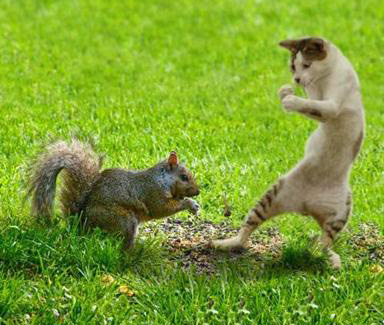
\includegraphics[width=0.5\textwidth]{squirrel}}
   \label{fig:squirrel}
\end{figure}
%\listoftodos
\section{Introduction}
In this assignment we focus on the learning scenario: the agents has no knowledge on the reward structure and the transition probabilities. We make a brief note about how we implemented relative state space, and make a concise comparison to the original state space on the performance improvements.

We then start by implementing Q-learning. We evaluate the effects of the various parameters on the steps taken per episode. We also visualize the Q-values to get a sense of what the algorithm learns.

Next we evaluate Softmax action selection, and compare it to $\epsilon$-greedy by evaluating the convergence-speed and the generated Q-values.

Lastly, we have implemented Sarsa, and compare it to Q-learning.
We briefly mention our implementation of On-Policy Monte-Carlo control which is not running optimally at the time of submission.

\subsection{Relative state space}
In assignment 1 we briefly described a potential state space reduction (see figure~\ref{fig:state_diagram}). We have implemented this new state space, which drastically decreases the computation time for the following experiments, especially since Q-learning has to loop over all the states. The absolute state space included one state for every possible combination of predator and prey positions. Since only the relative distance between the players determines the choice of the action to be taken by the predator, we now only encode the Manhattan distance in the state representation.

We illustrate in figure~\ref{fig:state_diagram} how the state would change, given an action of the predator and the stochastic movement of the prey. Say the predator is at location 5,5 and the prey at 7,8 in the 11x11 grid. We would then encode the state as (2,3). If the predator then moves down, and the prey moved up, the new state would be (0,3). 
\begin{figure}[h!]
	\centering
    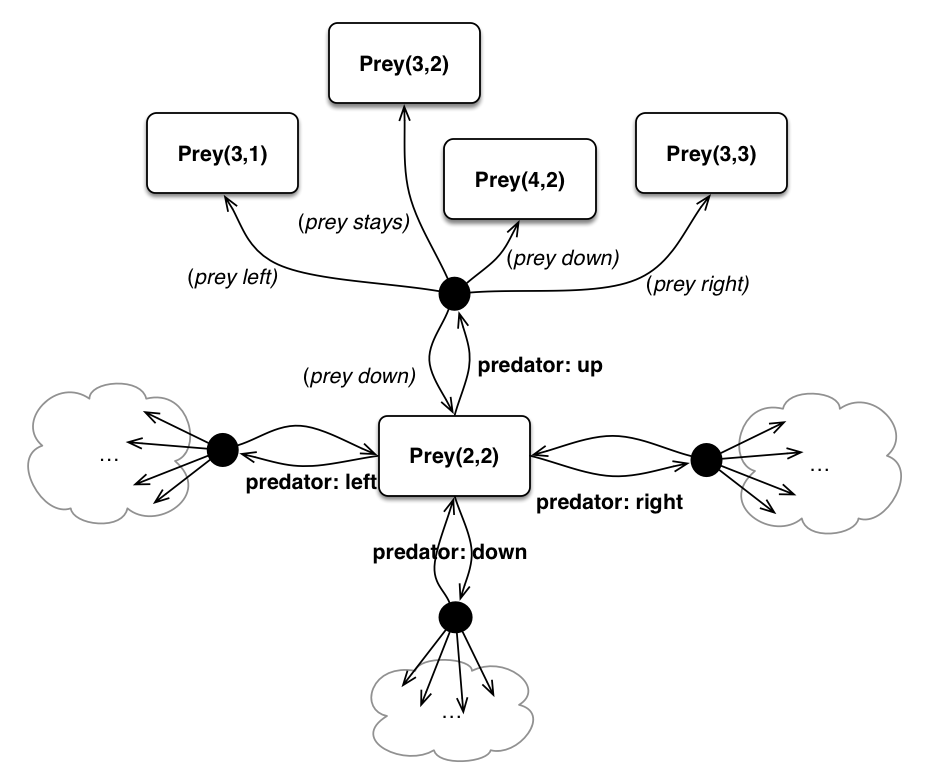
\includegraphics[width=0.75\textwidth]{state_diagram}
  \caption{State diagram for relative position}
   \label{fig:state_diagram}
\end{figure}
\section{Q-learning}
The first algorithm we will evaluate is Q-learning. This is implemented in ^q\_learning.py^ and plotting in ^graphics/plot\_qlearning\_graphs.py^. 
To evaluate the effect of the parameters, we take combinations of the parameter values and run the Q-learning algorithm for 15,000 episodes. We consider two performance measures. The primary focus lies on the percentage of correct greedy-actions based on the current Q-value. However, if we care about episode length during learning, we use the steps taken per episode as a measure of the agent's performance.

Because the prey moves randomly, the number of steps per episode varies greatly, even after training. To visualize the convergence of Q-learning properly, we plot a moving average of 1000 episodes and 0.2 $\times$ stdev (the area around the line) over this 1000-episode window. We do the same averaging for the correct percentage, for easier comparison.

\subsection{Learning rate $\alpha$}
We start by evaluating different values for the learning rate $\alpha$. We fix the discount factor $\gamma$ to 0.7 and pick $\alpha$ from \{0.05, 0.1, 0.5, 0.9\}. The results are shown in figure~\ref{fig:qlearning-lr}. We see two effects of the learning rate parameter. Lower learning rates result in slower convergence, higher learning rates in more variance and levels off at a lower value.
This is further illustrated by figure~\ref{fig:qlearning-lr_radical} which shows that Q-learning with $\alpha=1$ keeps altering its policy.

\begin{figure}[h!]
	\centering
    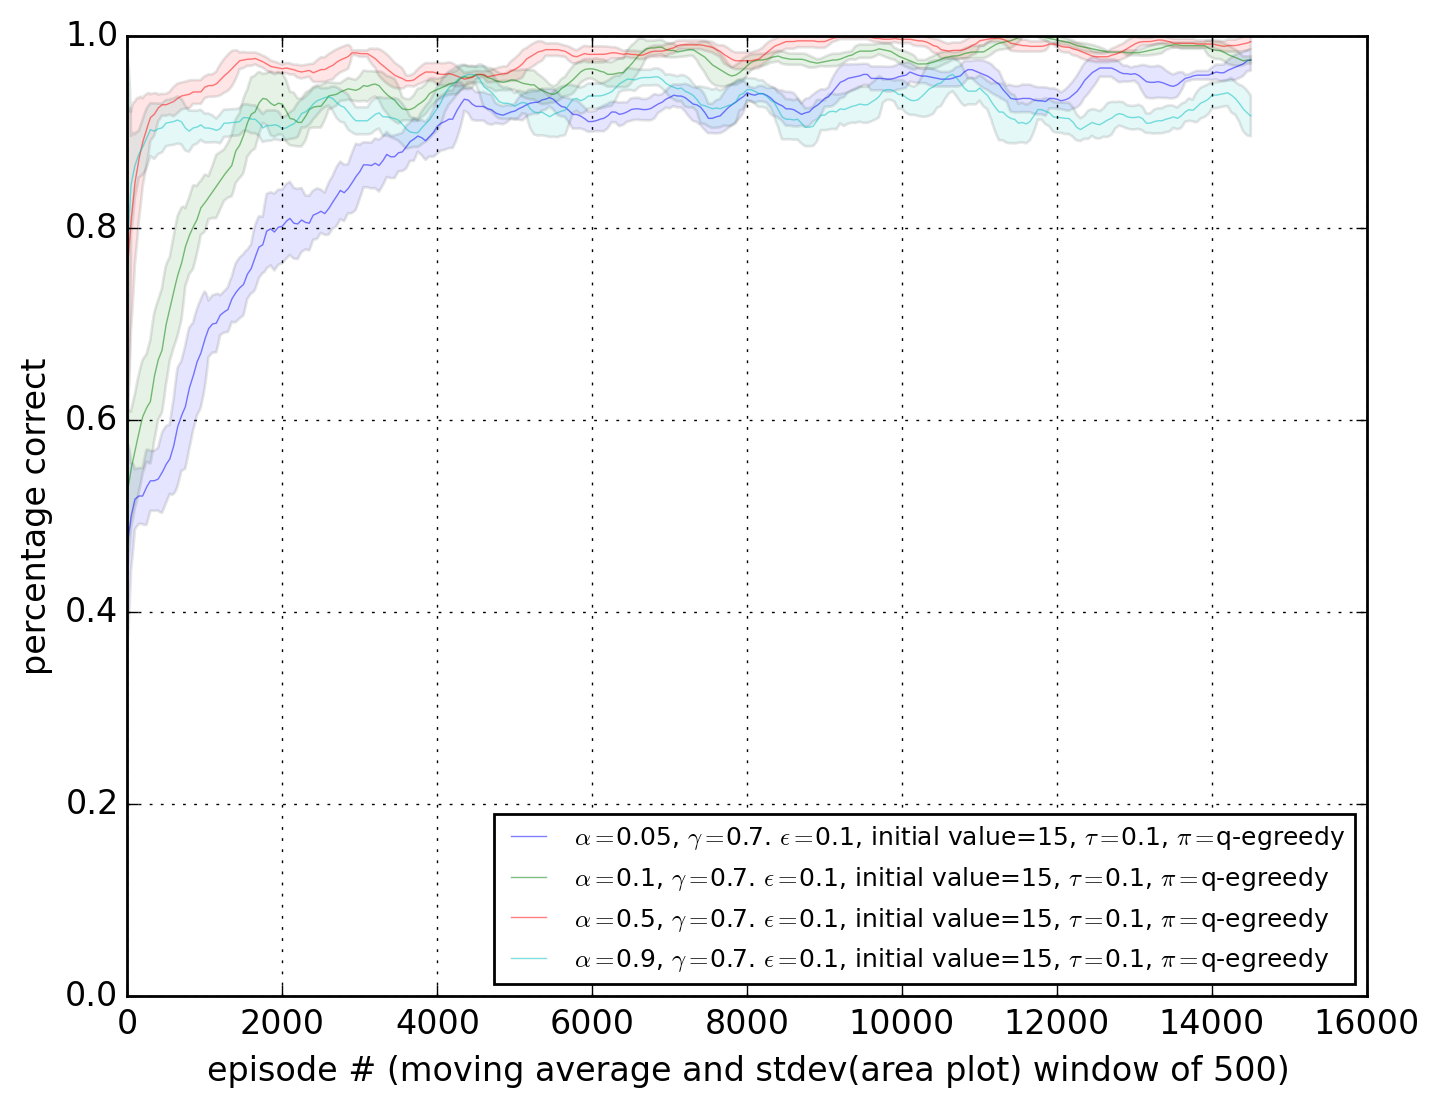
\includegraphics[width=.85\textwidth]{qlearning-lr}
  \caption{Convergence of Q-learning for different learning rate values}
   \label{fig:qlearning-lr}
\end{figure}

\begin{figure}[h!]
	\centering
    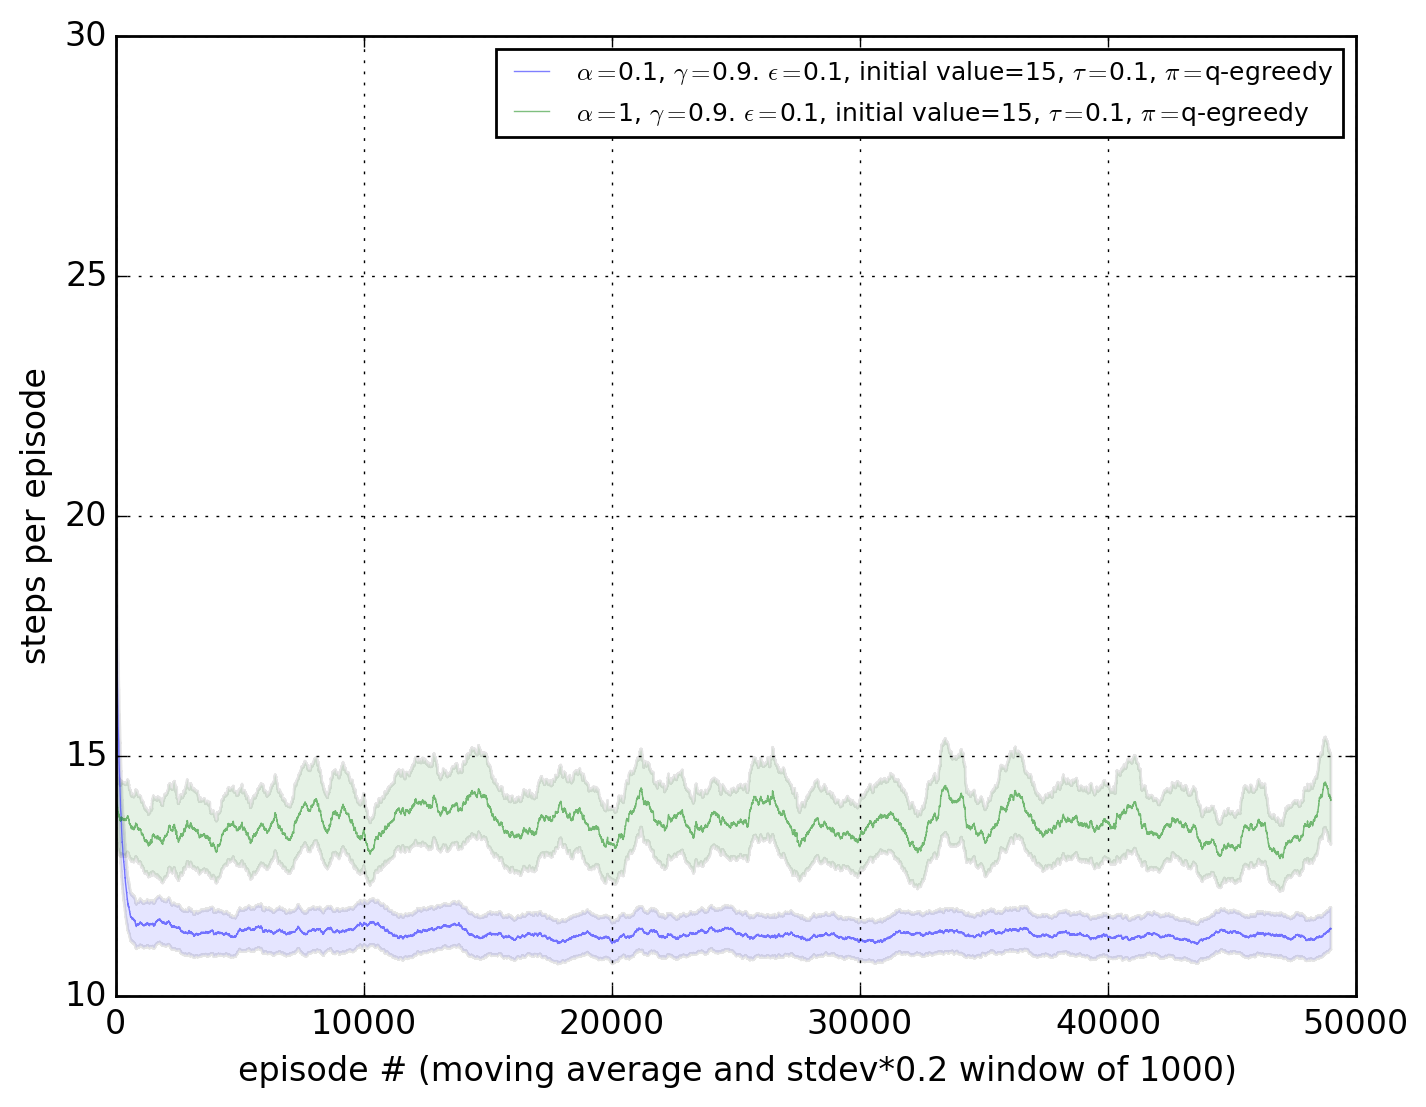
\includegraphics[width=.85\textwidth]{qlearning_lr_radical}
  \caption{Q-learning with 50.000 steps with a very high and a very low $\alpha$}
   \label{fig:qlearning-lr_radical}
\end{figure}

\subsection{Discount factor $\gamma$}
Next we evaluate the effect of the discount factor on the performance convergence. We fix the learning rate to 0.1, since this is a stable learning rate according to our previous experiment. We then pick discount factors of \{0, 0.1, 0.5, 0.7,0.9, 1\} and run a similar experiment as in the last subsection. The results are shown in figure~\ref{fig:qlearning-df}. The first conclusion we can make from this graph is that both extreme values 0 and 1 for the discount factor result in no learning at all. This is to be expected, because a discount factor of 0 means that the reward is attributed to only the most recent action, so no value is learned for the steps leading up to catching the prey. A discount factor of 1 means that the reward is equally attributed to all actions taken in an episode so far, so wrong actions taken earlier in the episode are valued positively for getting the final reward.

The less extreme values \{0.1, 0.5, 0.7,0.9\} show more subtle differences. The higher values converge faster, are more stable and more optimal in general. The result indicates that a discount factor of .9 is optimal.
\begin{figure}[h!]
	\centering
    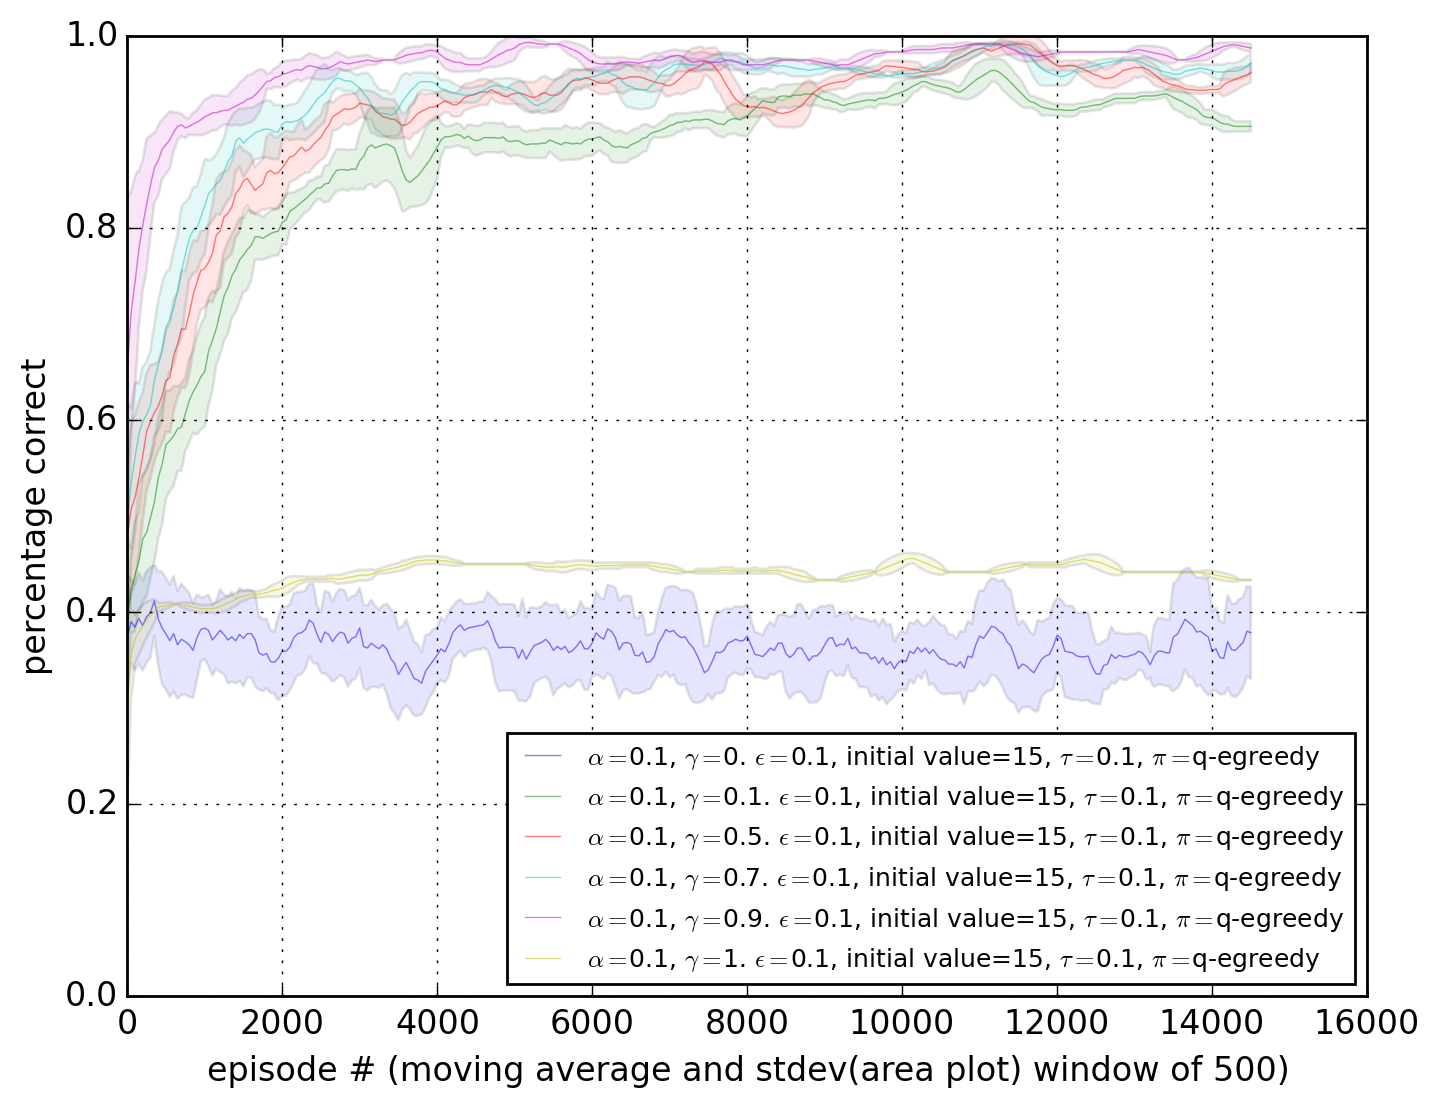
\includegraphics[width=.85\textwidth]{qlearning-df}
  \caption{Convergence of Q-learning for different discount factor values}
   \label{fig:qlearning-df}
\end{figure}

\subsection{Q-values evaluation}
In order to evaluate the correctness of the algorithm, we look at the actions a greedy q-value policy would take. We plot the maximizing action given a fixed prey location in the center and variable predator locations in figure~\ref{fig:qvalues}. The arrow length indicates the Q-value, and the direction is the maximizing action. This makes it plausible that our Q-learning implementation correctly converges to the optimal values.
\begin{figure}[h!]
	\centering
    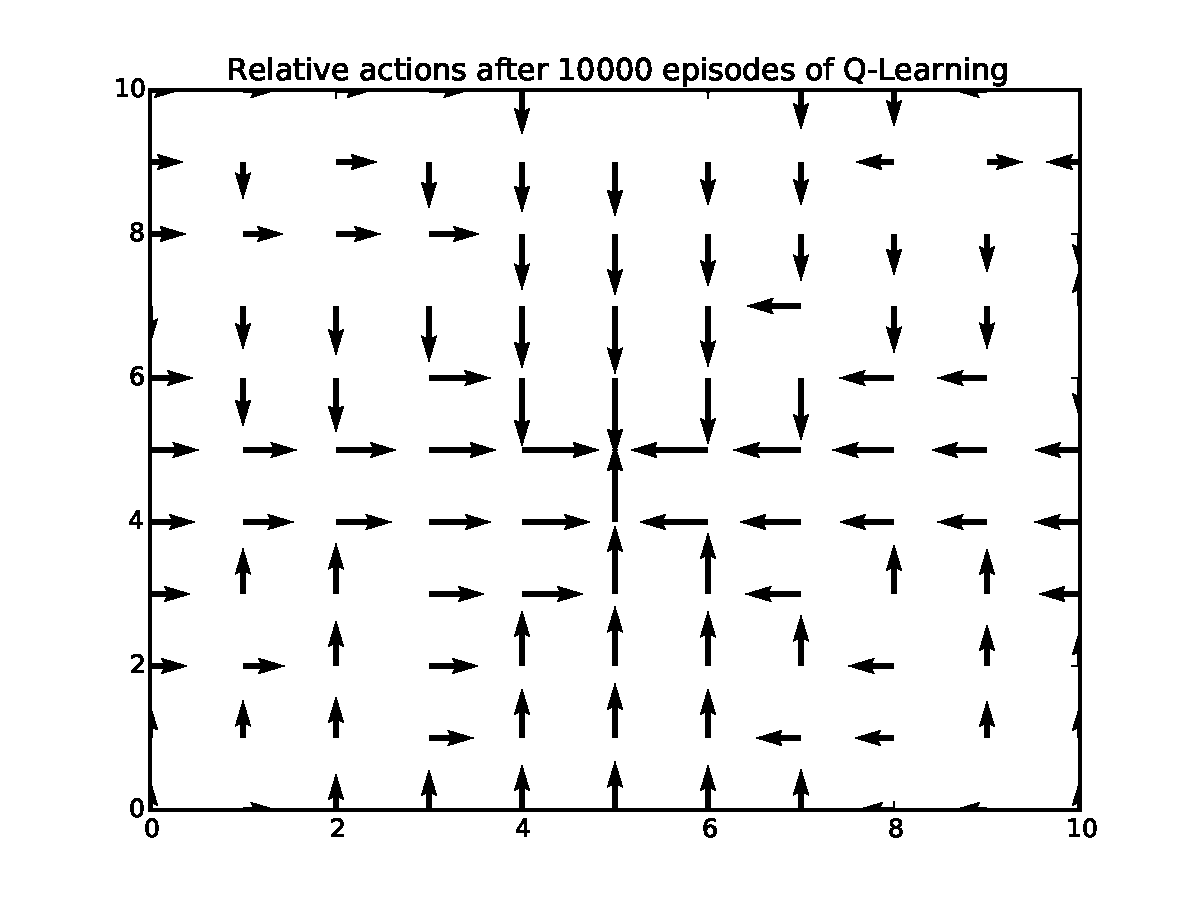
\includegraphics[width=0.6\textwidth]{qlearning-arrows.pdf}
  \caption{Learned optimal actions for the relative state space (prey sits in the center) after 10,000 episodes with $\alpha=0.1$, $\gamma=0.9$ and $\epsilon=0.1$.}
   \label{fig:qvalues}
\end{figure}

\section{Optimal Epsilon and optimistic initialization values}
Epsilon is the chance of picking a non-greedy action using the $\epsilon$-greedy policy. In order to find an optimal value, we evaluate $\epsilon=$\{0.05,0.1,0.2\} combined with optimistic initialization values of 5 and 15. We choose these values because 15 is higher than the final reward, which results in a high incentive to explore all state/action pairs. 5 is lower than the final reward, but will still results in some incentive to explore state/action pairs that only appear in the beginning of the episode. These have a lower value during training, due to the discounting factor.

The results are shown in figure~\ref{fig:epsilon-optimistic} (Please take note of the lower range on the y-axis, which was changed for clarity). The graph shows that initial values of 5 result in faster convergence but level of slower. This is expected, because the algorithm has to spend less time on exploring less-optimal state/action pairs, but will also miss some optimal ones.

Higher values of epsilon converge both faster and seem to perform better. One could expect higher values to often deviate from the optimum due to higher chances of exploring sub-optimal actions, but this does not appear to be the case.
\begin{figure}[h!]
	\centering
    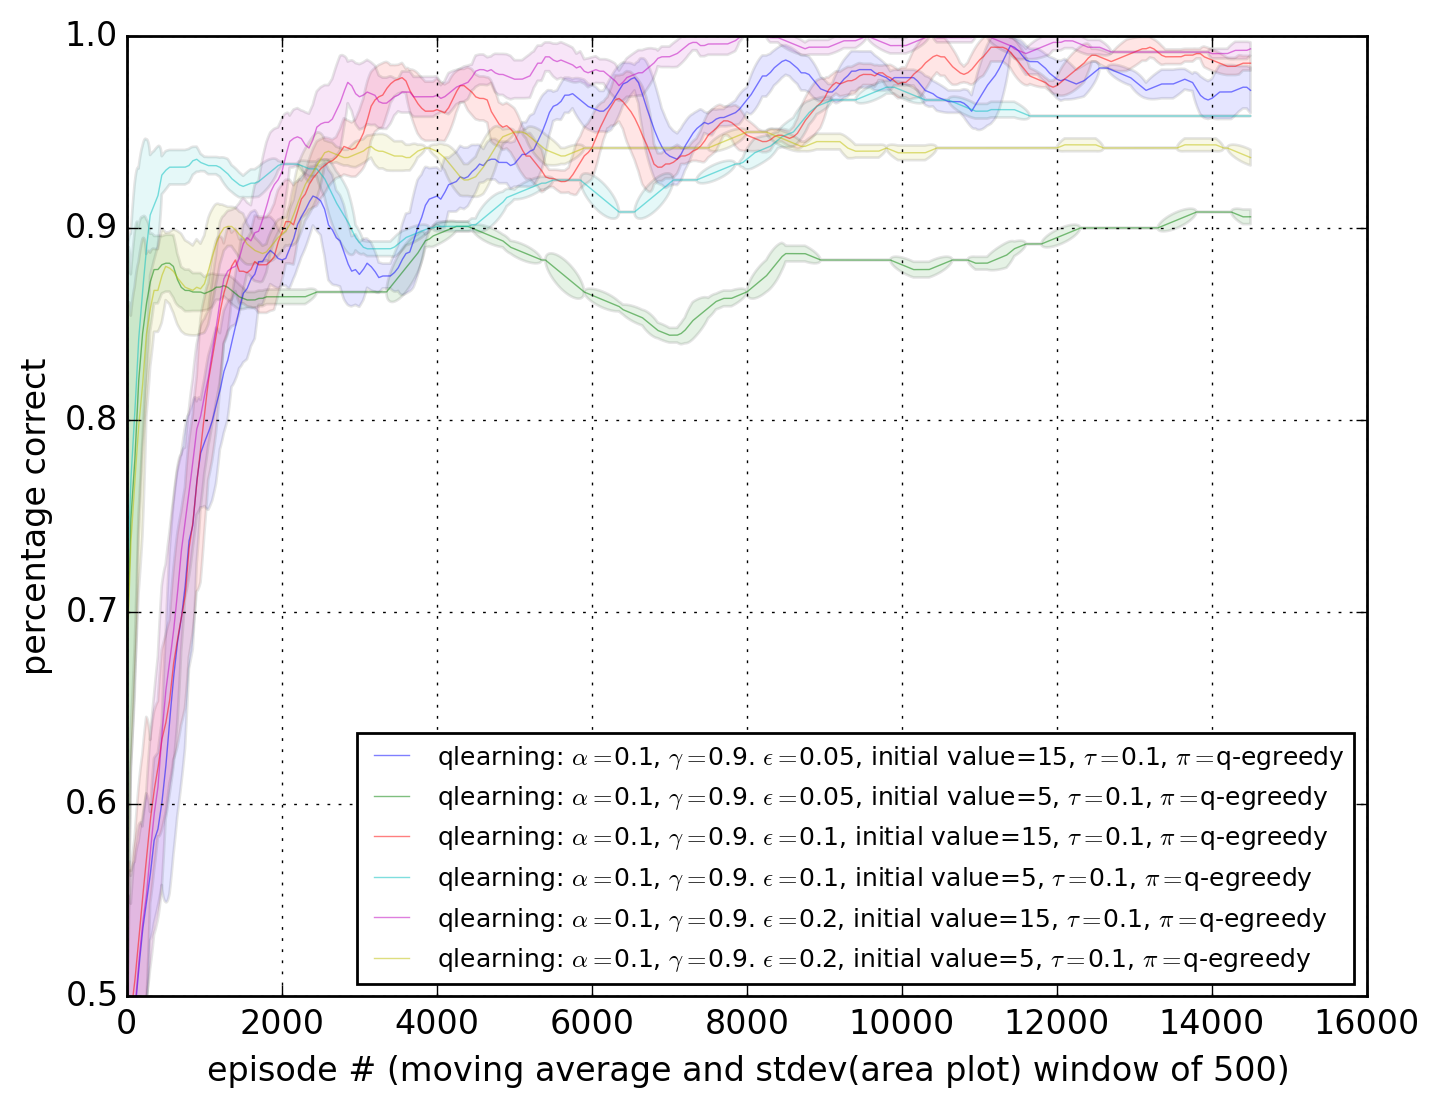
\includegraphics[width=.9\textwidth]{epsilon-optimistic}
  \caption{Convergence of Q-learning for different epsilon and initial values}
   \label{fig:epsilon-optimistic}
\end{figure}

In order to validate the assumption that higher values of epsilon perform worse considering the steps per episode during learning, we run another experiment with a fixed initial value of 15 and epsilon values of 0.1, 0.2 and  0.5, shown in figure~\ref{fig:high-epsilon}. This shows that higher epsilon values take more steps per episode during learning, which both increases the computation time and the average reward per time step during learning. 

Depending on whether your goal is computing optimal Q-values or getting the highest reward during learning, high epsilon values are good or bad, respectively. 
\begin{figure}[h!]
	\centering
    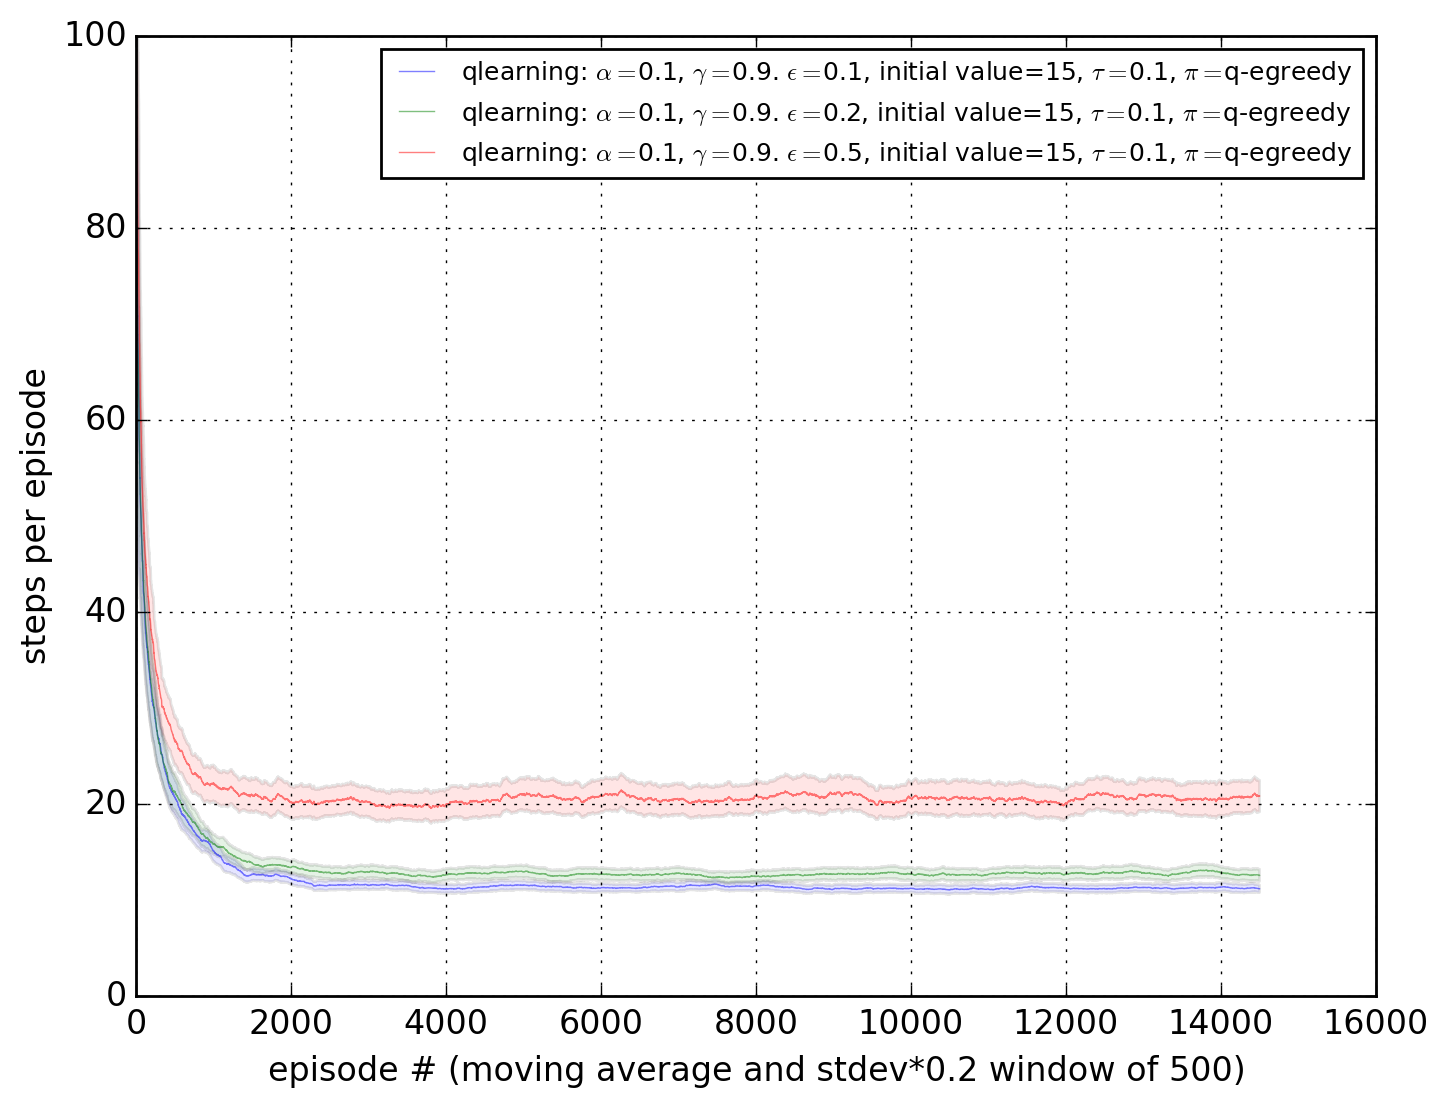
\includegraphics[width=.9\textwidth]{high-epsilon}
  \caption{Convergence of Q-learning for high epsilon values}
   \label{fig:high-epsilon}
\end{figure}
\section{Softmax action selection}
Softmax is implemented in ^policy.py^. We first evaluate values of $\tau$ to find the optimum. The results are shown in figure~\ref{fig:softmax-tau}. We see that higher values of tau converge faster to the optimum q-values. However, they explore more during learning, resulting in more steps per episode on average with higher variance. This also results in more information per episode, explaining part of the reason why higher tau values converge to the optimum in less episodes. From this we conclude that picking $\tau$ depends on the goal of the learning step, with lower values resulting in higher performance during learning, but taking more time to find the optimal values.

Next we compare softmax to $\epsilon$-greedy with fixed parameters using $\tau=0.1$. The results are shown in figure~\ref{fig:softmax}. The plots show that softmax converges to the optimal value faster and does not deviate from it like $\epsilon$-greedy does. This indicates that softmax performs better during learning (although converging slightly slower in the beginning).
\begin{figure}[h!]
	\centering
    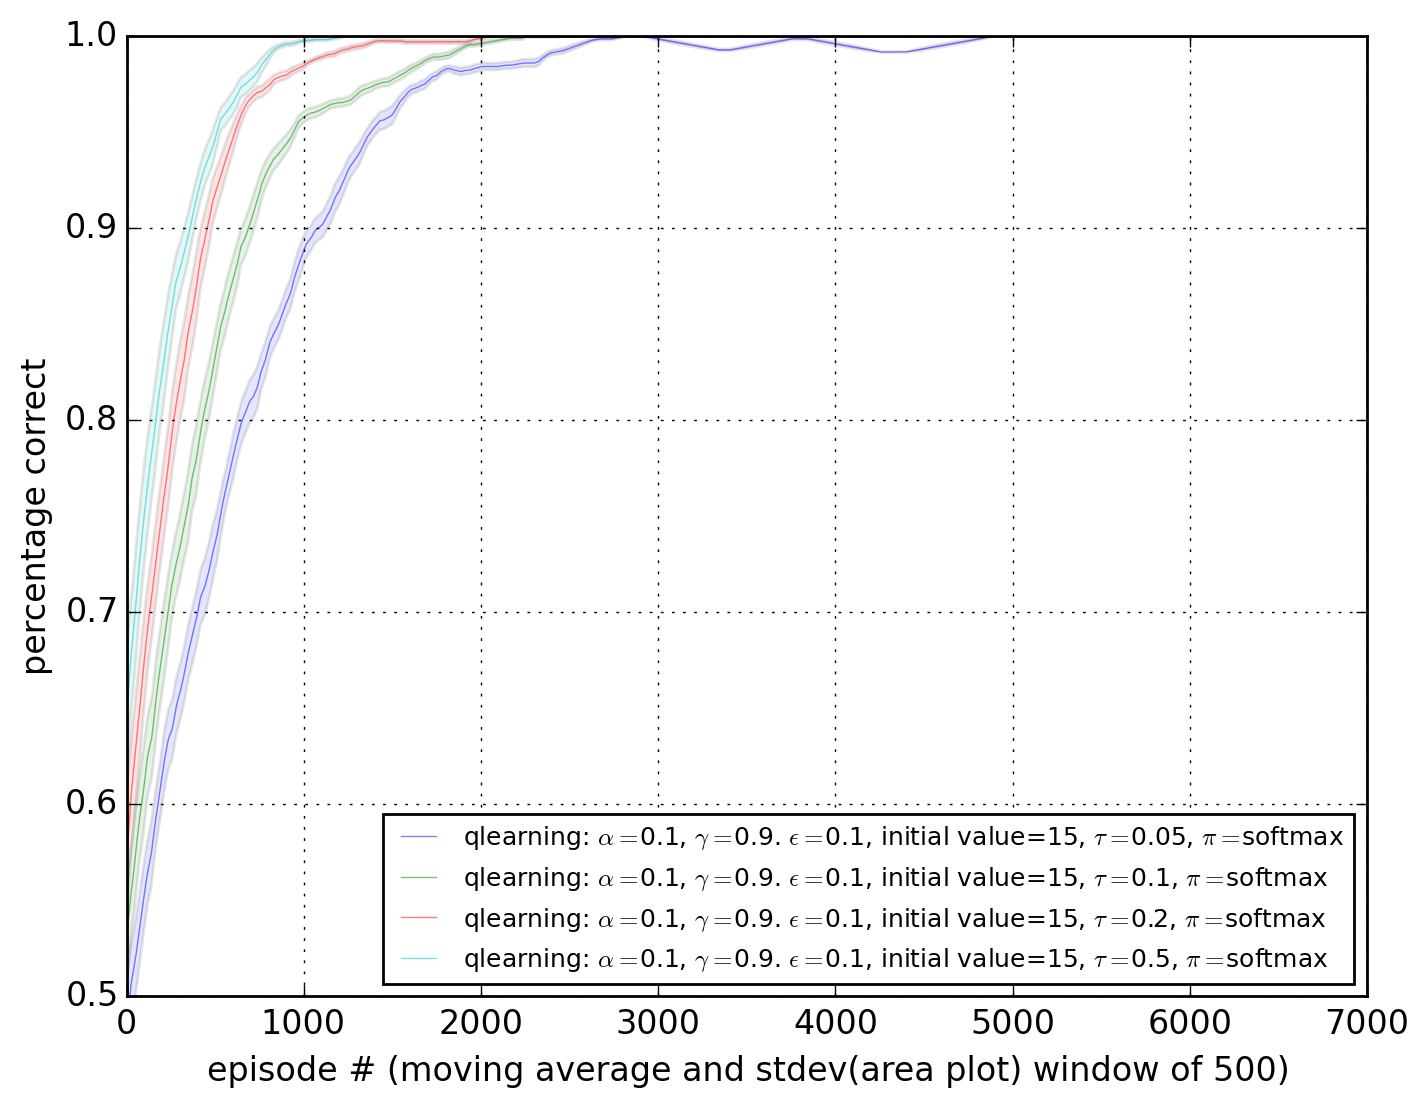
\includegraphics[width=.45\textwidth]{softmax-tau-perc}
    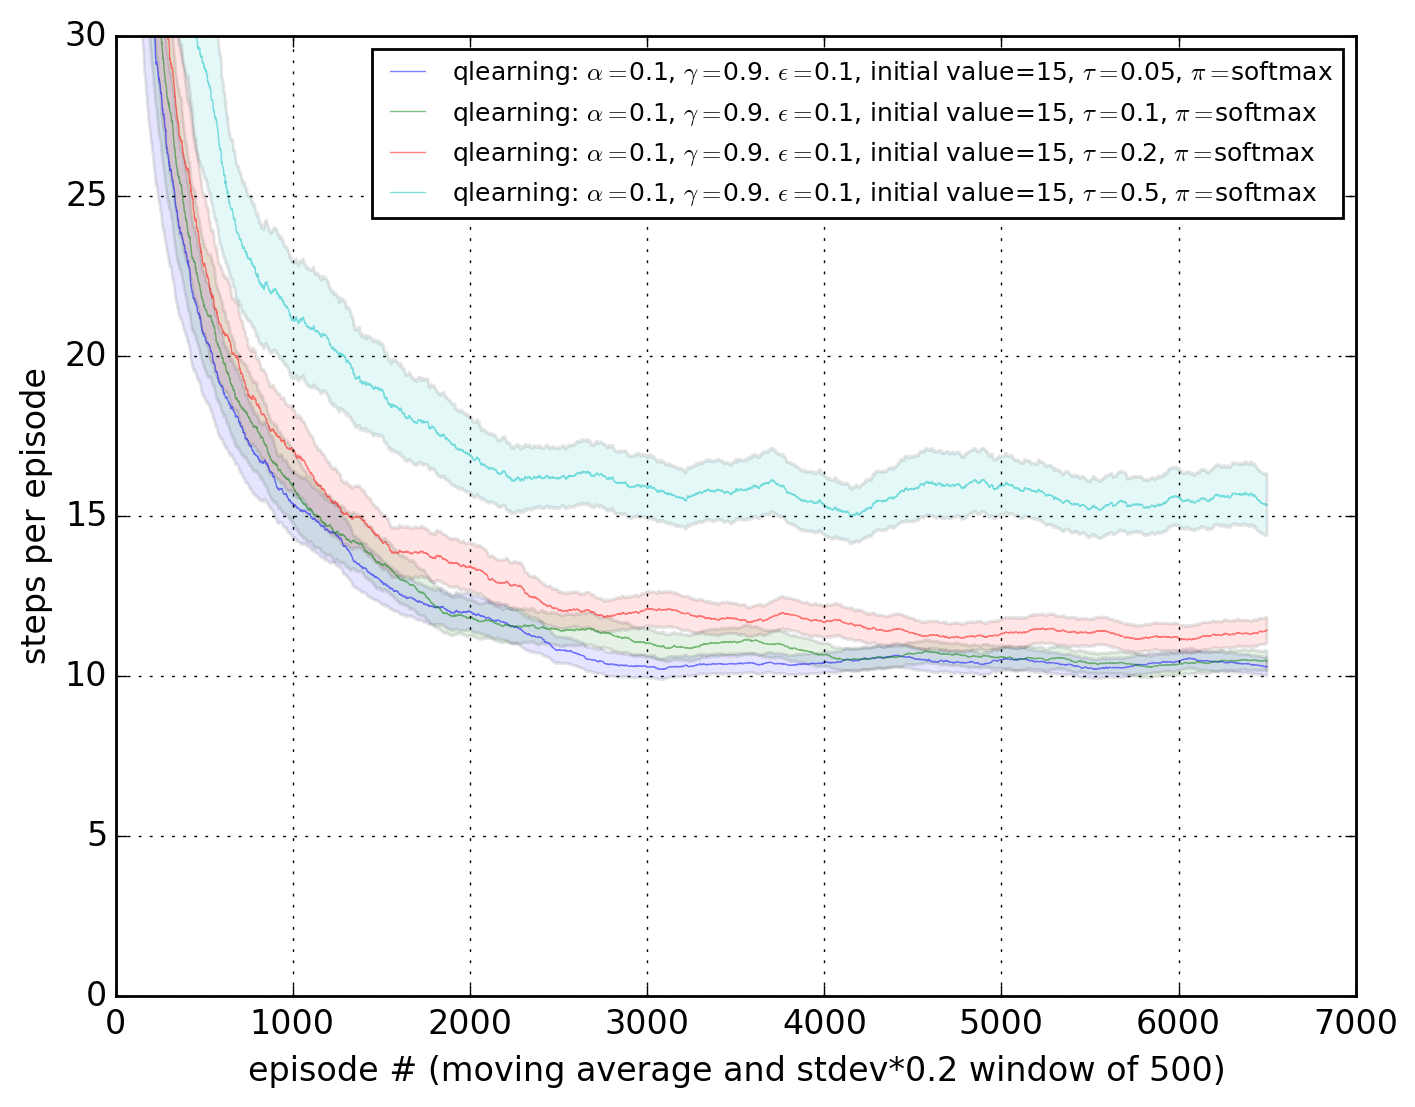
\includegraphics[width=.45\textwidth]{softmax-tau-steps}
  \caption{Softmax: evaluating values of $\tau$}
   \label{fig:softmax-tau}
\end{figure}
\begin{figure}[h!]
	\centering
    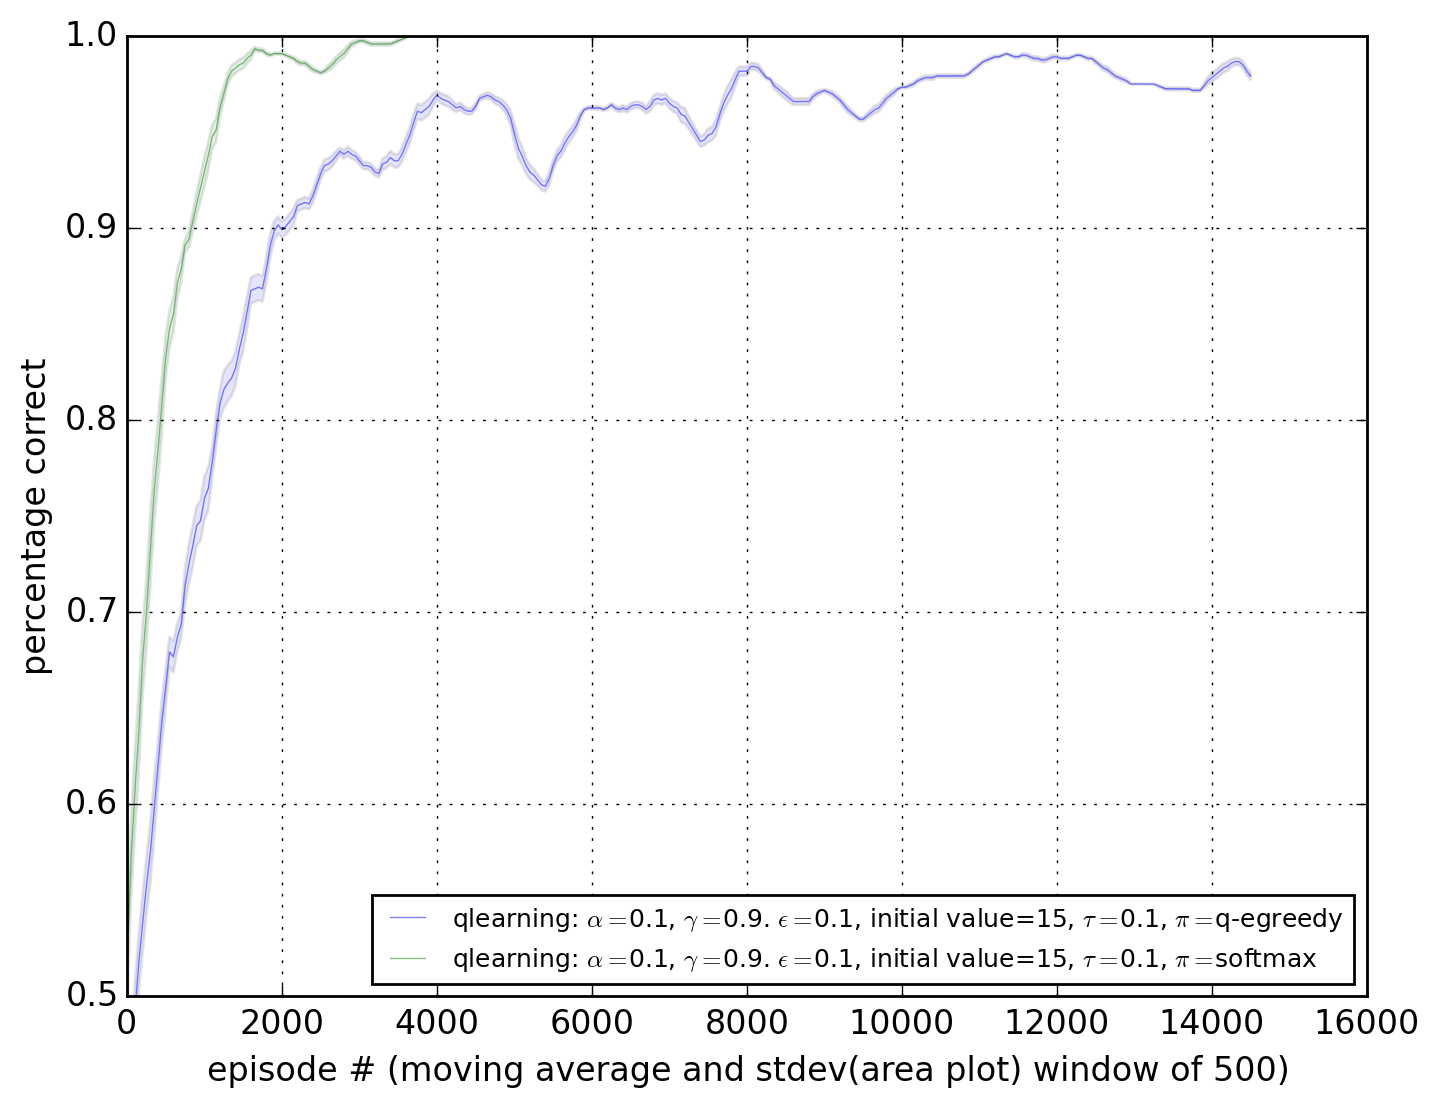
\includegraphics[width=.45\textwidth]{softmax-perc}
    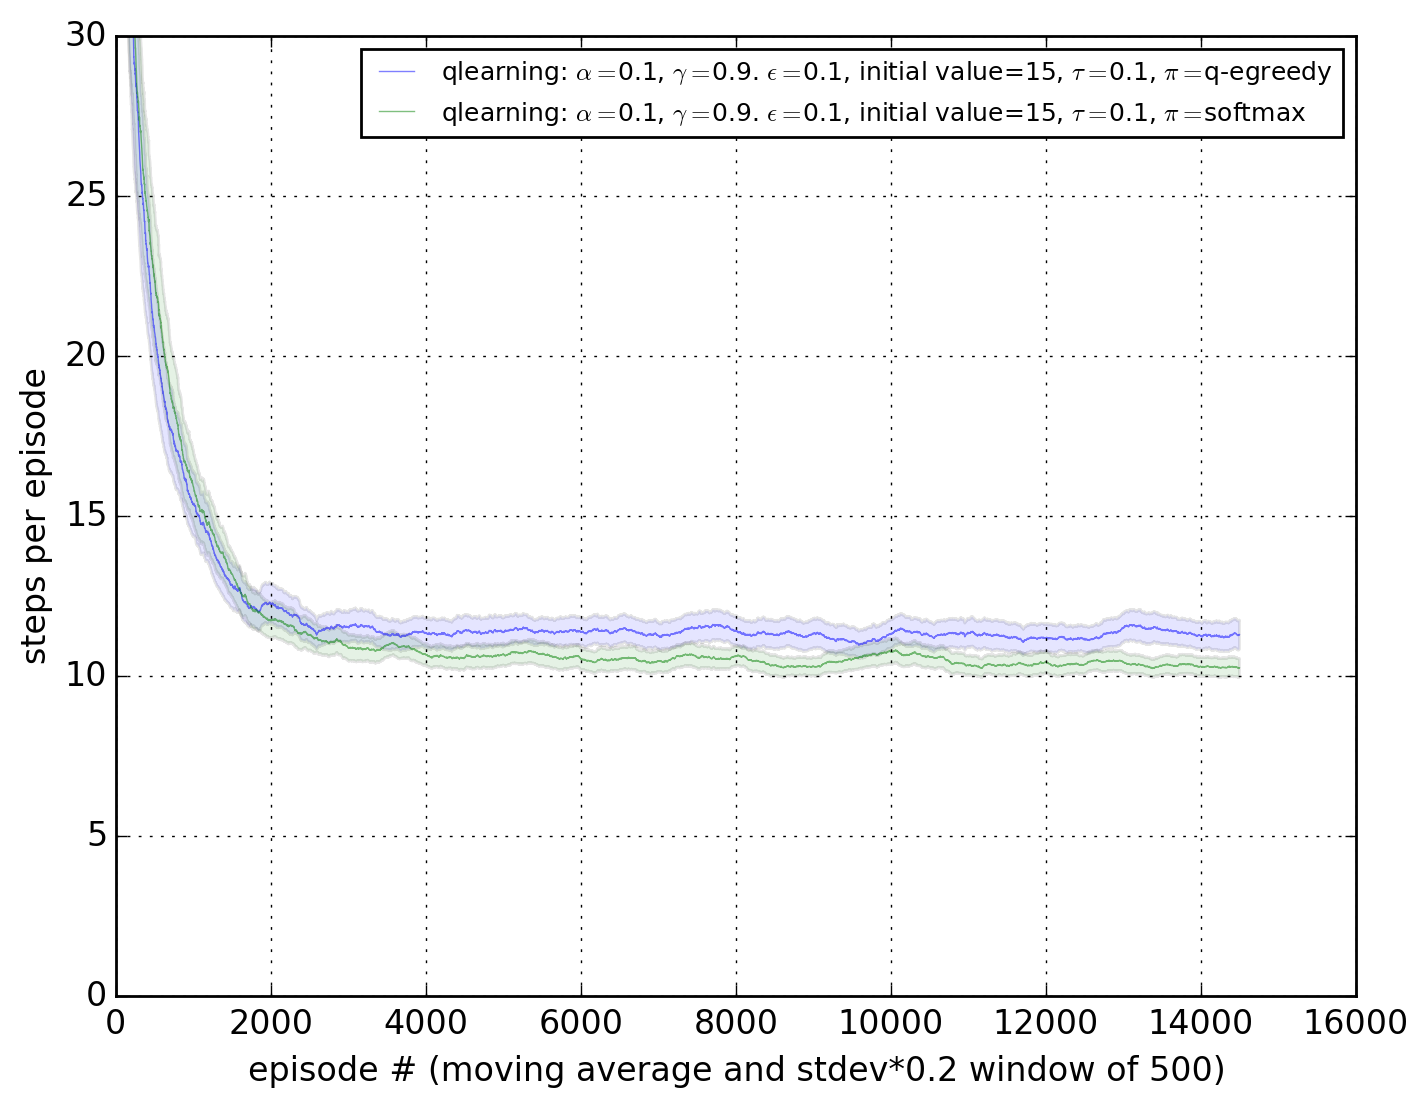
\includegraphics[width=.45\textwidth]{softmax-steps}
  \caption{Softmax versus $\epsilon$-greedy: percentage correct and steps taken}
   \label{fig:softmax}
\end{figure}


\section{Sarsa}
Sarsa is implemented in ^sarsa.py^. We evaluate our implementation by simply comparing Sarsa to Q-learning with fixed parameters. The results are shown in figure~\ref{fig:sarsa}. From the results we can
conclude that our implementation of sarsa performs similar to q-learning (this is also the case for an $\epsilon$-greedy policy). 

\begin{figure}[h!]
	\centering
    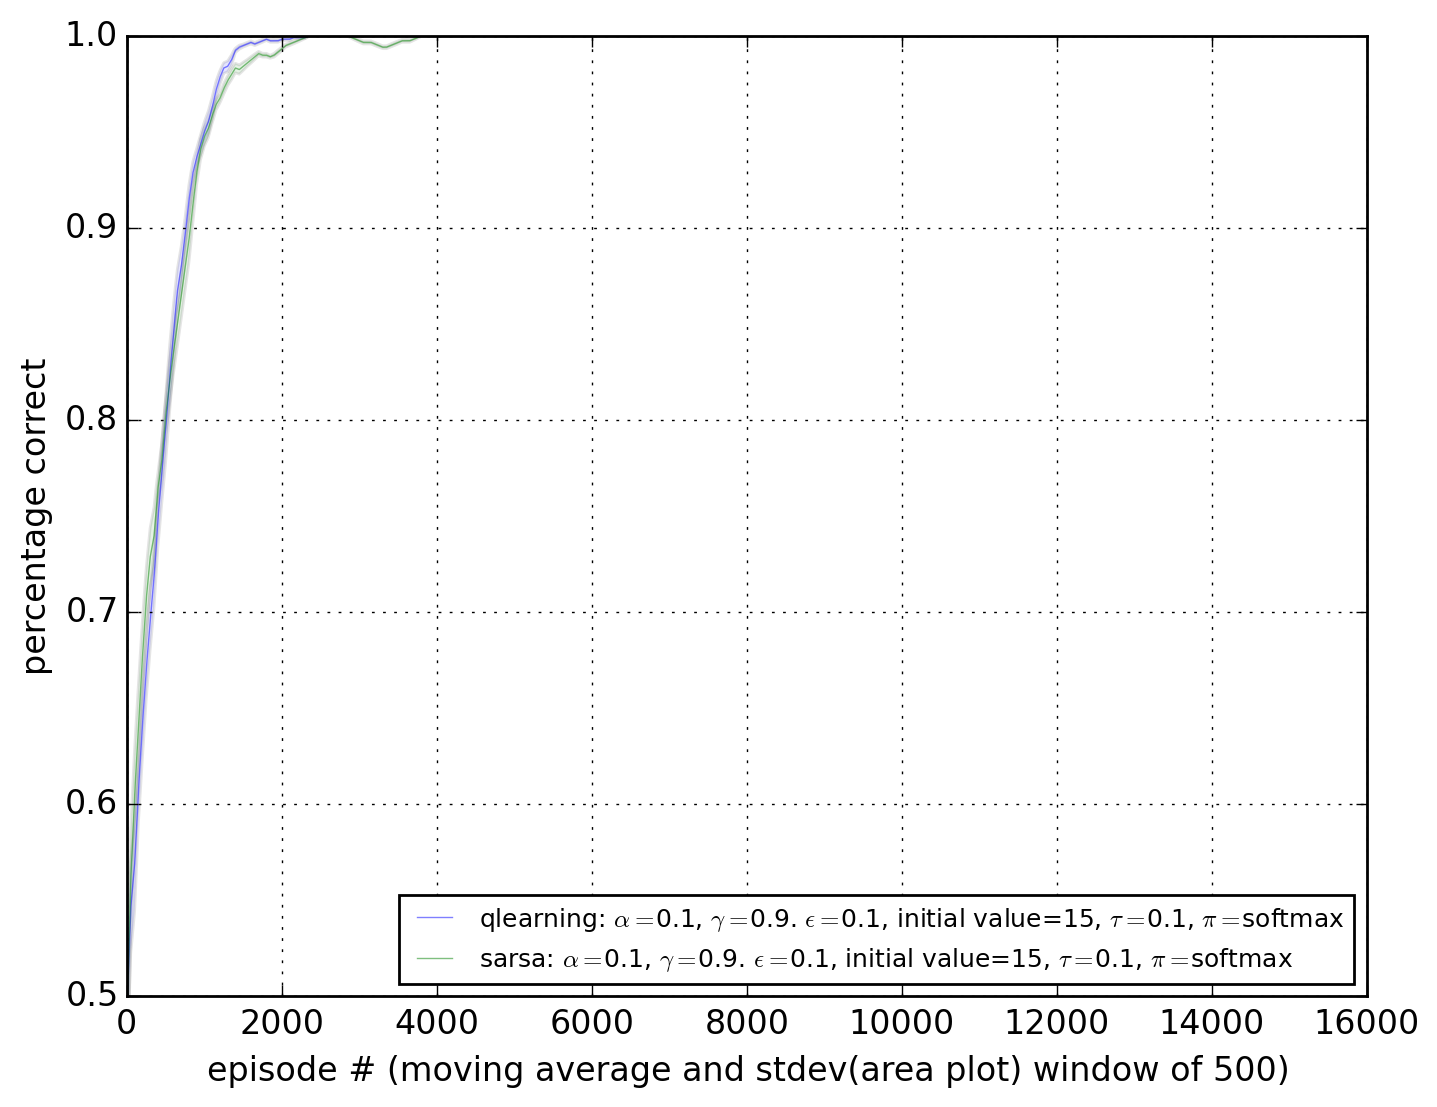
\includegraphics[width=.45\textwidth]{sarsa-perc}
    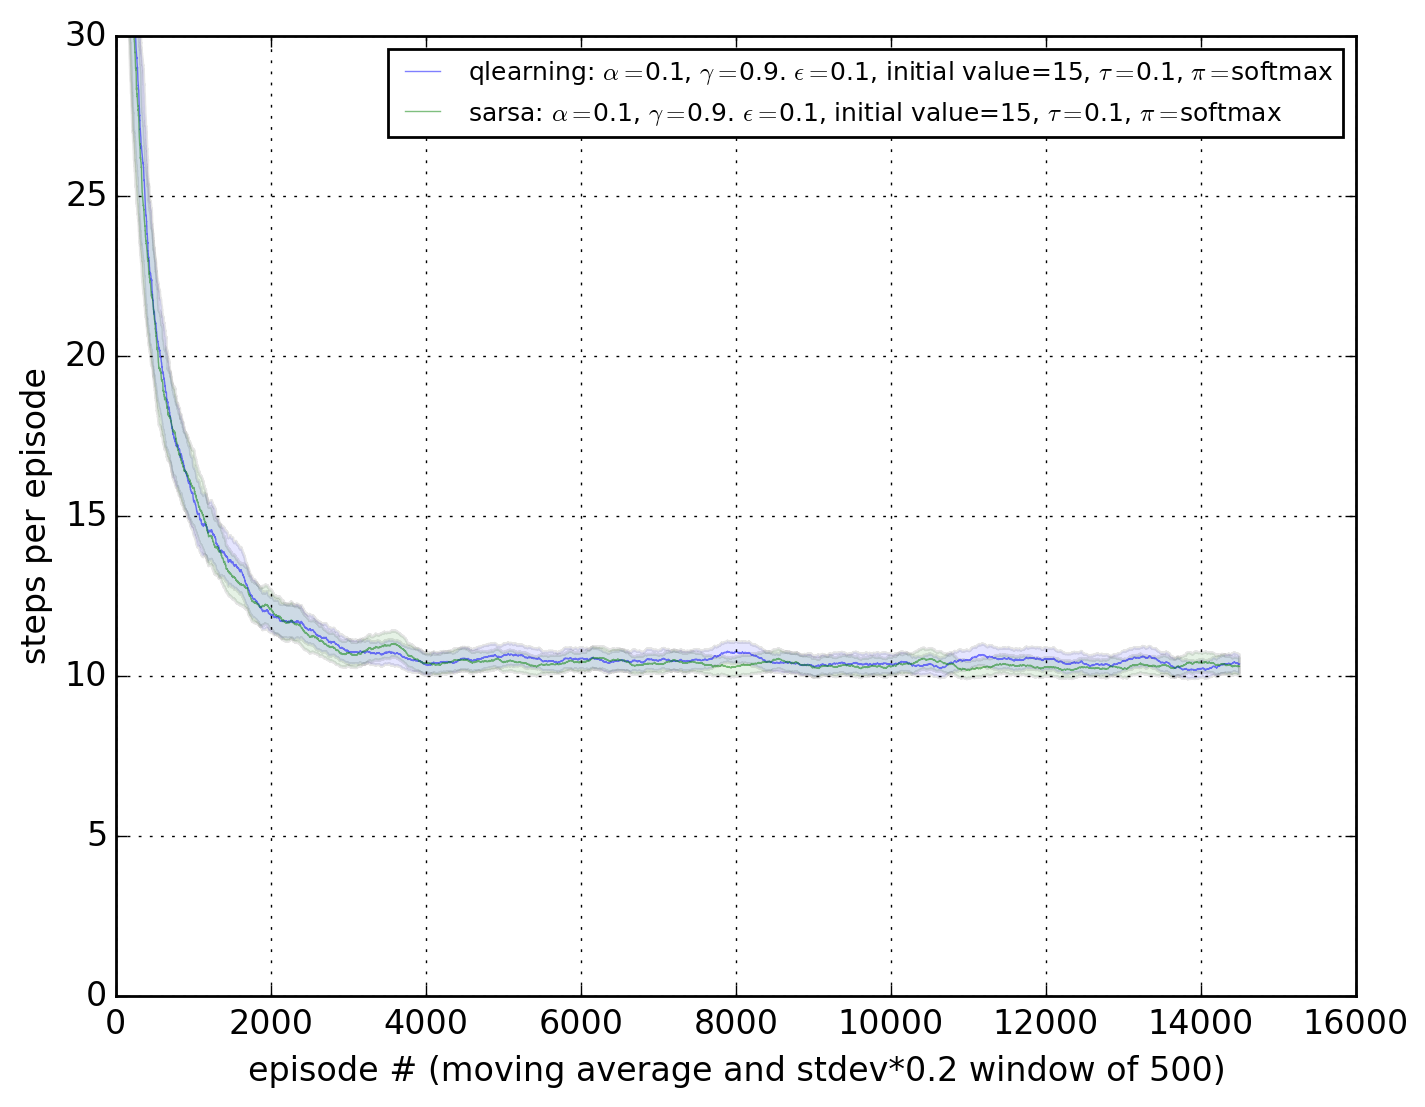
\includegraphics[width=.45\textwidth]{sarsa-steps}
  \caption{Sarsa versus Q-learning: percentage correct and steps taken}
   \label{fig:sarsa}
\end{figure}

\subsection{Visualizing the algorithm}
In order to easily grasp which policy results from learning in Sarsa (and also other algorithms), we introduced an animated GUI that visualizes the path taken by each player per episode. By setting the ^gui=True^ flag when running either of the algorithms, it will simulate one episode in the GUI after the training. A screenshot of the window after 10,000 training episodes in Sarsa is shown in figure~\ref{fig:gui_sarsa}. The red trace denotes the path taken by the predator, the blue line for the prey. We can see that the predator (depicted by a cat icon) went almost straight towards the prey (squirrel icon) and caught it in the red colored box. 


\begin{figure}[h!]
	\centering
    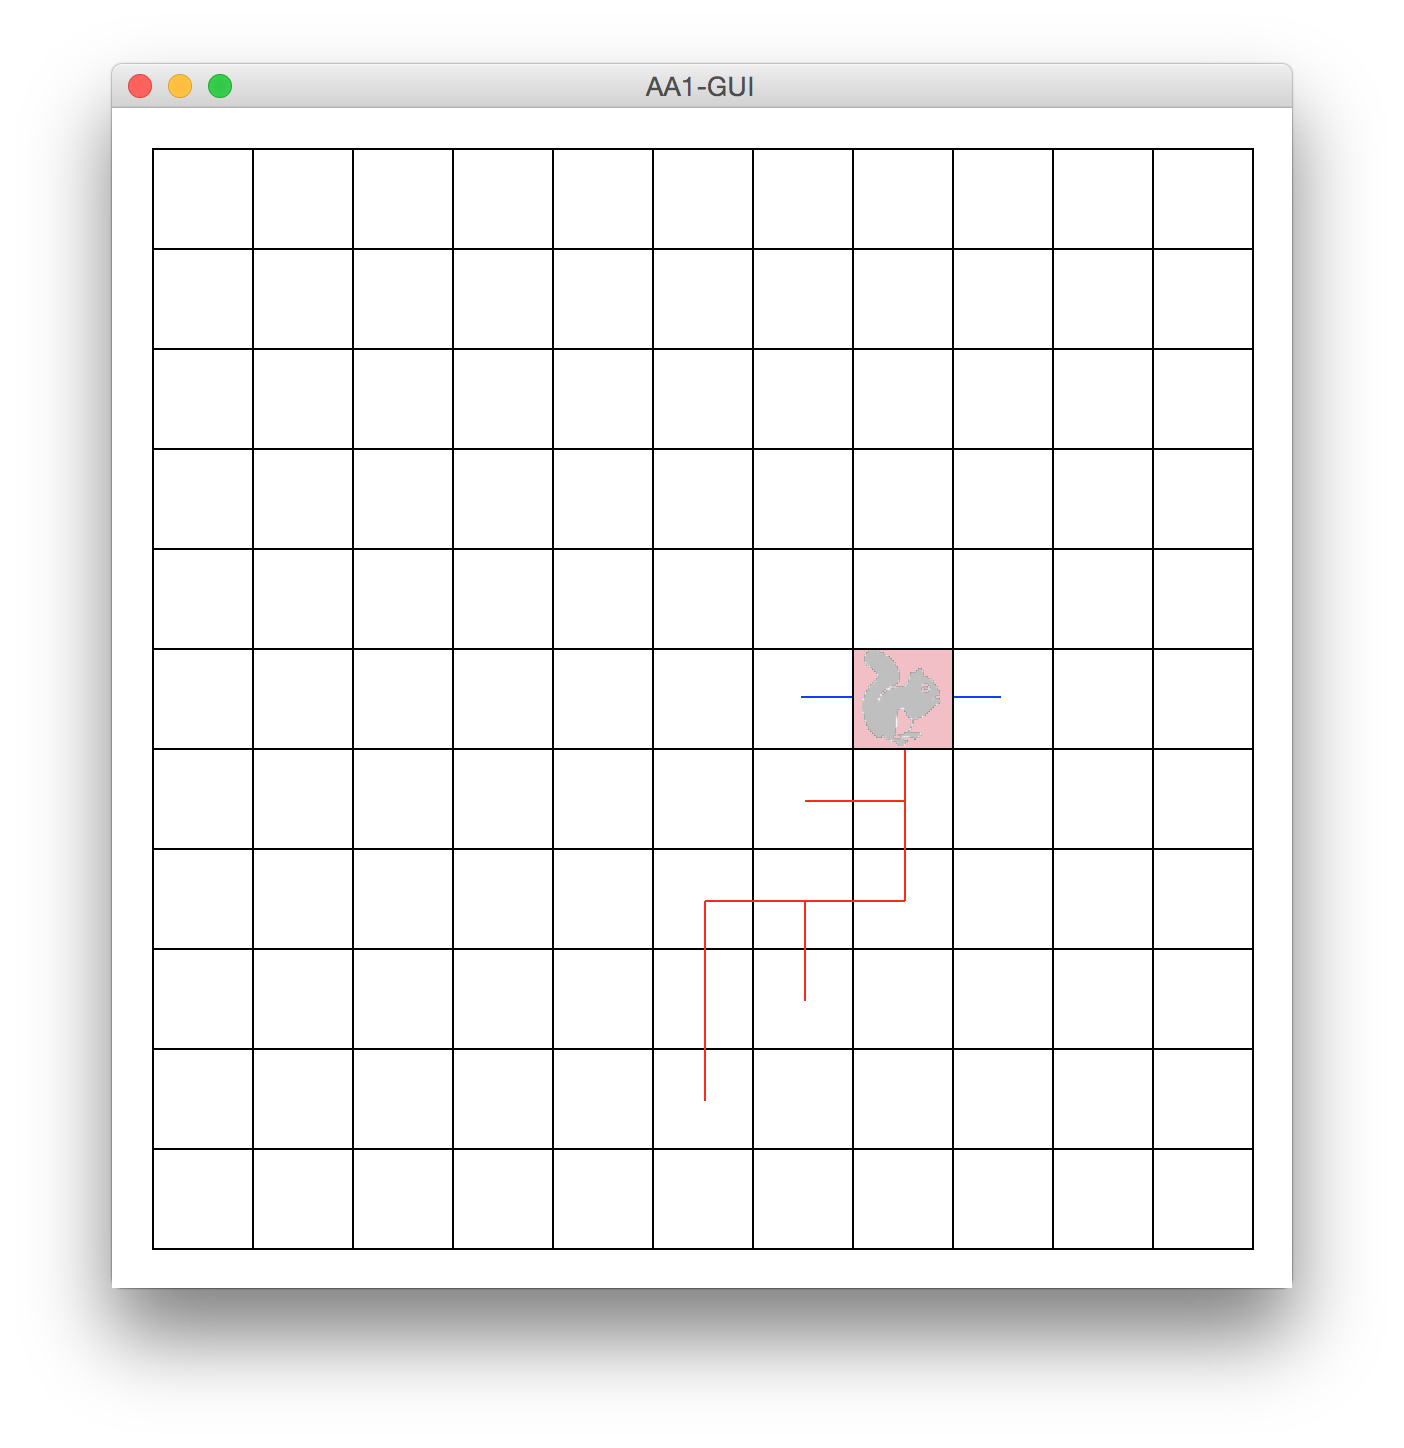
\includegraphics[width=.5\textwidth]{gui_sarsa_10000}
    \caption{Graphical User Interface for visualization of the learning algorithms}
   \label{fig:gui_sarsa}
\end{figure}

\section{On-Policy Monte Carlo Control}
The On-Policy Monte-Carlo control algorithm can be found in ^on\_policy\_evaluation.py^. 
Note that our implementation of the algorithm still has some issues. If we chose too small values of Q and the policy took a suboptimal action in a random state in the beginning, but did not visit the state again, the agent will continue to select this inferior action as the greedy choice and did it more often than choosing a probably better action. \\
We got better results when introducing a discount factor on the return values. Normally it is enough to take the average of the summed up rewards, divided by the amount of episodes taken. But since the reward is only generated at the very end of each episode and then propagated back instead of in-between rewards during the episode, it should do nothing more than just give a steeper slope to the right action. This should result in faster learning.\\
The resulting plot of the average steps-per-episode in figure \ref{fig:onpolicyrun}, shows that the algorithm performs poorly without converging the steps-per-episode average or variance.

\begin{figure}[h!]
	\centering
    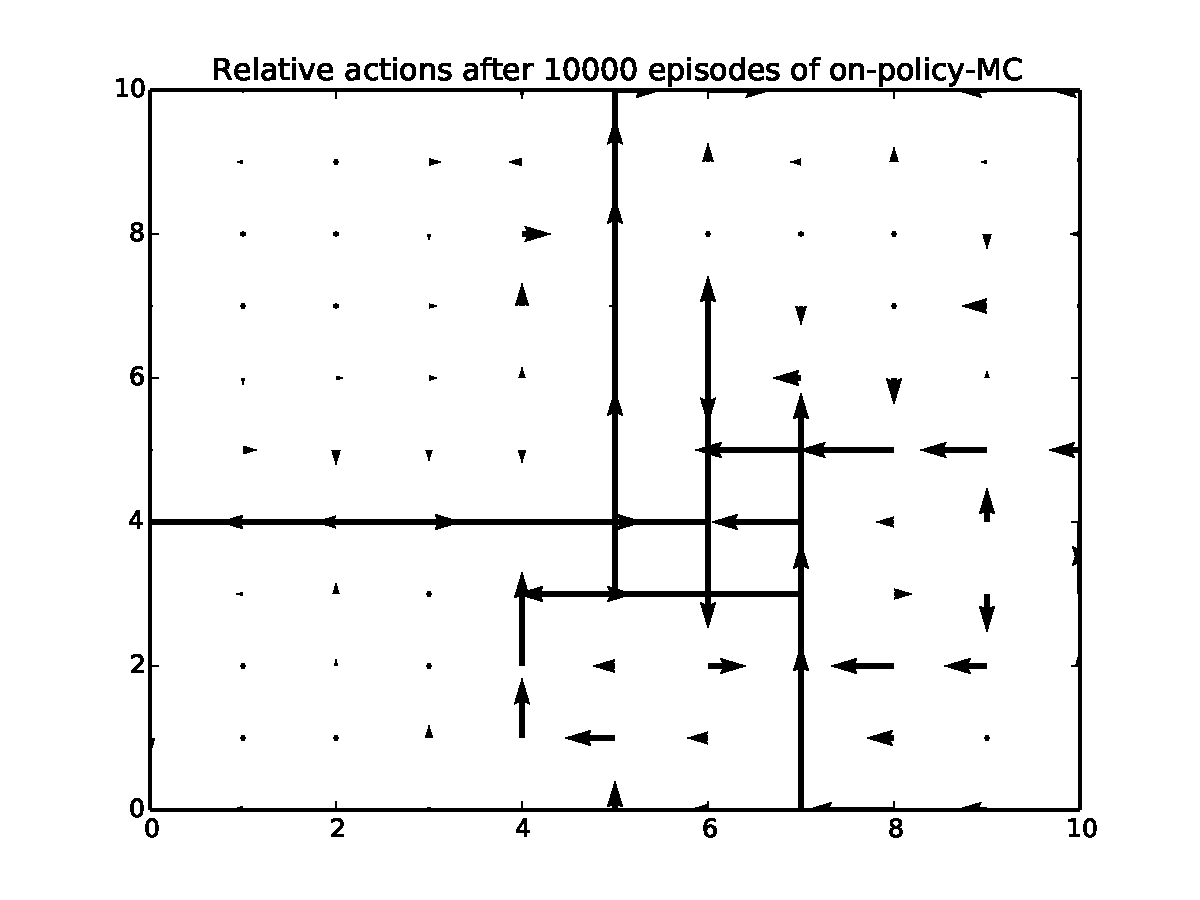
\includegraphics[width=.6\textwidth]{onpolicymc_arrows}
   % \includegraphics[width=.45\textwidth]{}
  \caption{The onpolicy MC results}
   \label{fig:onpolicy-mc}
\end{figure}
\begin{figure}[h!]
	\centering
    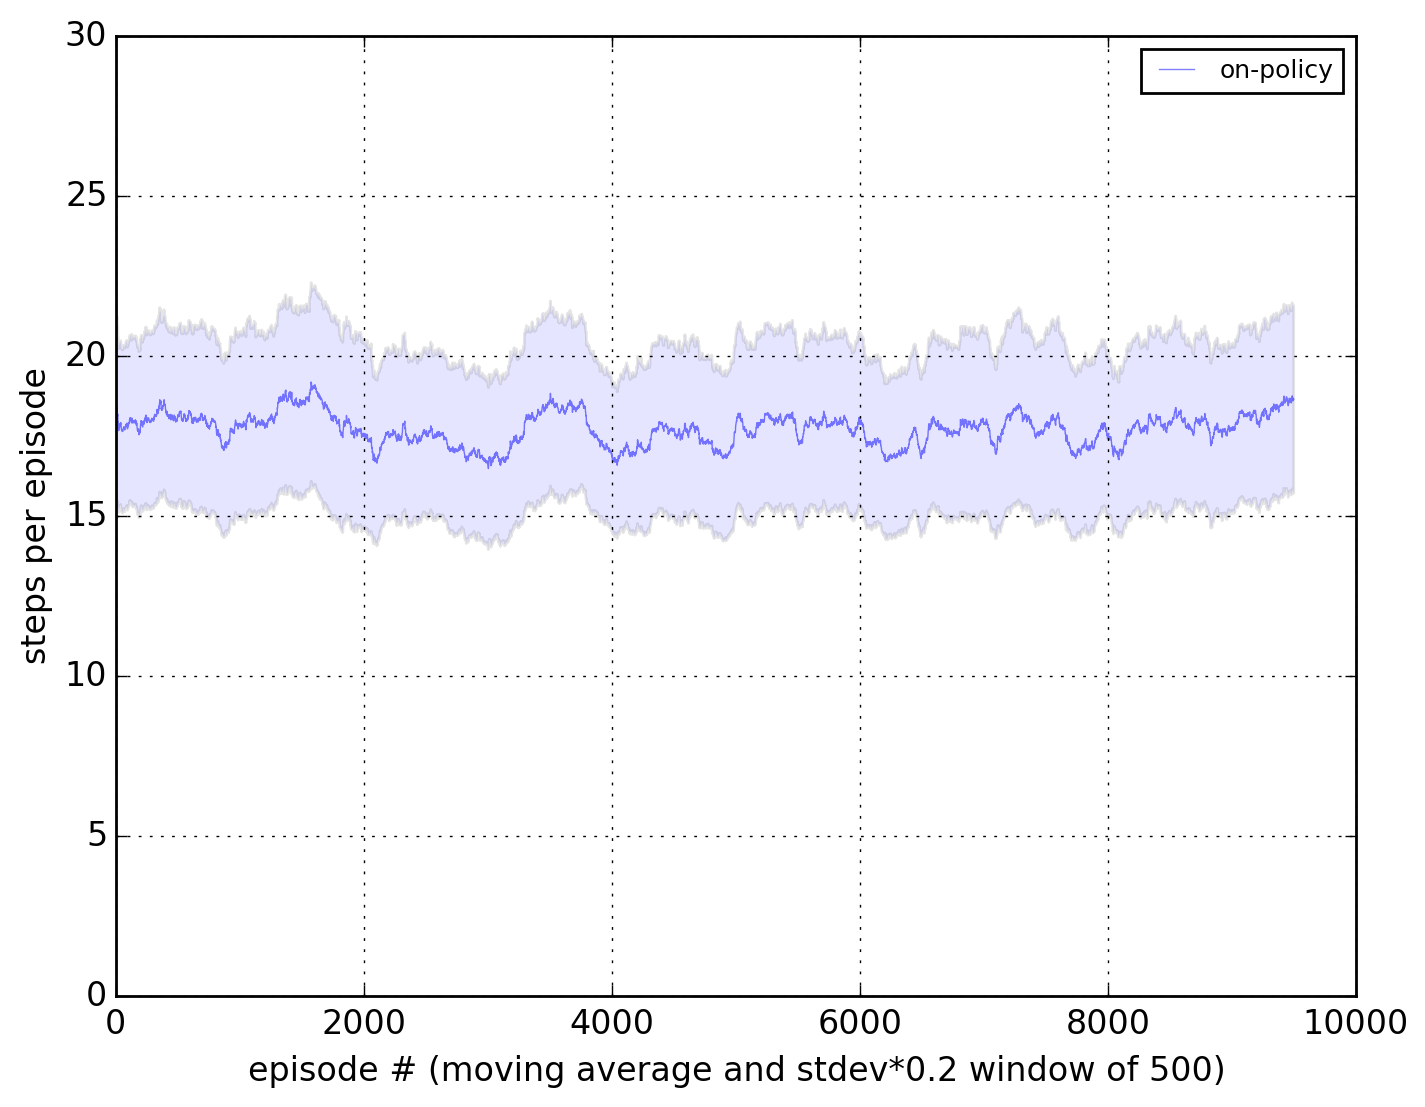
\includegraphics[width=.9\textwidth]{onpolicy}
  \caption{On-Policy Monte Carlo Control run}
   \label{fig:onpolicyrun}
\end{figure}

\section{Conclusion}
In this assignment, we explored Q-learning and the effect of its various parameters in a Predator-Prey problem. We have shown empirically that lower learning rates result in slower convergence but to a more correct Q-value. Higher values of the  discount factor result in better performance, but some discounting is required for the algorithm to converge swiftly.

The initial values of Q and epsilon  influence the performance of Q-learning as well. Empirical results show that high values of epsilon converge closer to the correct Q-values, but result in poor performance during training. Decreasing the initial values below the actual reward results in less exploration and thus a lower bound on the correctness.

Using the Softmax policy increase the convergence speed and results in perfect Q-values. Furthermore it results in less steps per episode on average. Higher values for the temperature parameter $\tau$ cause more exploration, and thus faster convergence to the optimum with worse performance per episode.

Comparing Q-learning to other learning algorithms, we found that our implementation of Sarsa performs similarly to Q-learning for the problem considered. Other learning algorithms introduced implementational difficulties.

Overall, the best performing algorithm was Q-learning using Softmax with a learning rate of 0.1, discount factor of 0.9, initial value of 15 and tau of 0.1.

\end{document}